\documentclass[a4paper,14pt]{extarticle}

\usepackage{cmap}
\usepackage[T2A]{fontenc}
\usepackage[utf8x]{inputenc}
\usepackage[english, russian]{babel}

\usepackage{misccorr} % в заголовках появляется точка, но при ссылке на них ее нет
\usepackage{amssymb,amsfonts,amsmath,amsthm}  
\usepackage{indentfirst}
\usepackage[usenames,dvipsnames]{color} 
\usepackage[unicode,hidelinks]{hyperref}
% \hypersetup{%
%     pdfborder = {0 0 0}
% }

\usepackage{makecell,multirow} 
\usepackage{ulem}
\usepackage{graphicx,wrapfig}
\graphicspath{{img/}}
\usepackage{geometry}
\geometry{left=2cm,right=2cm,top=3cm,bottom=3cm,bindingoffset=0cm,headheight=15pt}
\usepackage{fancyhdr} 
\linespread{1.05} 
\frenchspacing 
\renewcommand{\labelenumii}{\theenumii)} 
\newcommand{\mean}[1]{\langle#1\rangle}
% \usepackage{caption}
%%%%%%%%%%%%%%%%%%%%%%%%%%%%%%%%%%%%%%%%%%%%%%%%%%%%%%%%%%%%%%%%%%%%%%%%%%%%%%%
%%%%%%%%%%%%%%%%%%%%%%%%%%%%%%%%%%%%%%%%%%%%%%%%%%%%%%%%%%%%%%%%%%%%%%%%%%%%%%%

\def\labauthors{Есюнин Д.В., Есюнин М.В.}
\def\labgroup{430}
% \def\department{Кафедра электроники и квантовой физики}
\def\labnumber{1}
\def\labtheme{Вынужденная синхронизация}

%%%%%%%%%%%%%%%%%%%%%%%%%%%%%%%%%%%%%%%%%%%%%%%%%%%%%%%%%%%%%%%%%%%%%%%%%%%%%%%
	%применим колонтитул к стилю страницы
\pagestyle{fancy} 
	%очистим "шапку" страницы
\fancyhead{} 
	%слева сверху на четных и справа на нечетных
\fancyhead[L]{\labauthors} 
	%справа сверху на четных и слева на нечетных
%\fancyhead[R]{Отчёт по лабораторной работе №\labnumber} 
	%очистим "подвал" страницы
\fancyfoot{} 
	% номер страницы в нижнем колинтуле в центре
\fancyfoot[C]{\thepage} 
\renewcommand{\phi}{\varphi}
%%%%%%%%%%%%%%%%%%%%%%%%%%%%%%%%%%%%%%%%%%%%%%%%%%%%%%%%%%%%%%%%%%%%%%%%%%%%%%%

\usepackage{float}
\usepackage[mode=buildnew]{standalone}
\usepackage{tikz} 
% \usepackage{subcaption}
\usepackage{tikz,csvsimple}
\usetikzlibrary{scopes}
\usetikzlibrary{%
     decorations.pathreplacing,%
     decorations.pathmorphing,%
    patterns,%
    calc,%
    scopes,%
    arrows,%
    % arrows.spaced,%
}
\makeatletter
\newif\if@gather@prefix 
\preto\place@tag@gather{% 
  \if@gather@prefix\iftagsleft@ 
    \kern-\gdisplaywidth@ 
    \rlap{\gather@prefix}% 
    \kern\gdisplaywidth@ 
  \fi\fi 
} 
\appto\place@tag@gather{% 
  \if@gather@prefix\iftagsleft@\else 
    \kern-\displaywidth 
    \rlap{\gather@prefix}% 
    \kern\displaywidth 
  \fi\fi 
  \global\@gather@prefixfalse 
} 
\preto\place@tag{% 
  \if@gather@prefix\iftagsleft@ 
    \kern-\gdisplaywidth@ 
    \rlap{\gather@prefix}% 
    \kern\displaywidth@ 
  \fi\fi 
} 
\appto\place@tag{% 
  \if@gather@prefix\iftagsleft@\else 
    \kern-\displaywidth 
    \rlap{\gather@prefix}% 
    \kern\displaywidth 
  \fi\fi 
  \global\@gather@prefixfalse 
} 
\newcommand*{\beforetext}[1]{% 
  \ifmeasuring@\else
  \gdef\gather@prefix{#1}% 
  \global\@gather@prefixtrue 
  \fi
} 
\makeatother

\usepackage{booktabs}
\usepackage{pgfplots, pgfplotstable}

\usepackage[outline]{contour}
\usepackage{tocloft}
\renewcommand{\cftsecleader}{\cftdotfill{\cftdotsep}} % for parts
% \renewcommand{\cftchapleader}{\cftdotfill{\cftdotsep}} % for chapters
\usepackage{pgfplots,pgfplotstable,booktabs,colortbl}
\pgfplotsset{compat=newest}
\usepackage{physics}
\usepackage{mathtools}
\mathtoolsset{showonlyrefs=true}
\newcommand\Smat{\hat { \mathbf { S } }}

\newcommand*\dotvec[1][1,1]{\crossproducttemp#1\relax}
\def\crossproducttemp#1,#2\relax{{\qty[\vec{#1}\times\vec{#2}\,]}}

\newcommand*\prodvec[1][1,1]{\crossproducttempa#1\relax}
\def\crossproducttempa#1,#2\relax{{\qty[{#1}\times{#2}\,]}}

% \def\E{\mathscr{E}_H}
\def\Rdim{\,\frac{\text{м}^3}{\text{А} \cdot \text{с}}}

\renewcommand{\vec}{\mathbf} % for parts


\begin{document}
	\begin{titlepage}

		\begin{center}
			
			
			\textsc{Нижегородский государственный университет имени Н.\,И. Лобачевского}
			\vskip 4pt \hrule \vskip 8pt
			\textsc{Радиофизический факультет}
			
			\vfill
			
			{\Large\labtheme}
			
		\end{center}
		
		\vfill
		
		\begin{flushright}
			{Работу выполнили студенты\\ \labauthors\\ 430 группы}
		\end{flushright}
		
		\vfill
		
		\begin{center}
			Нижний Новгород, \the\year
		\end{center}
	\end{titlepage}
%	\tableofcontents
	\newpage 
\section*{Экспериментальное исследование синхронизации}
\subsection*{Описание установки}
На рис. \ref{pic.1} приведены общий вид и схема экспериментальной установки для изучения явления вынужденной синхронизации. Установка состоит из: синхронизируемого автогенератора с изменяемым коэффициентом возбуждения (1), генератора силы регулируемой частоты и амплитуды (2), осциллографа (3).
\begin{figure}[H]
	\centering
	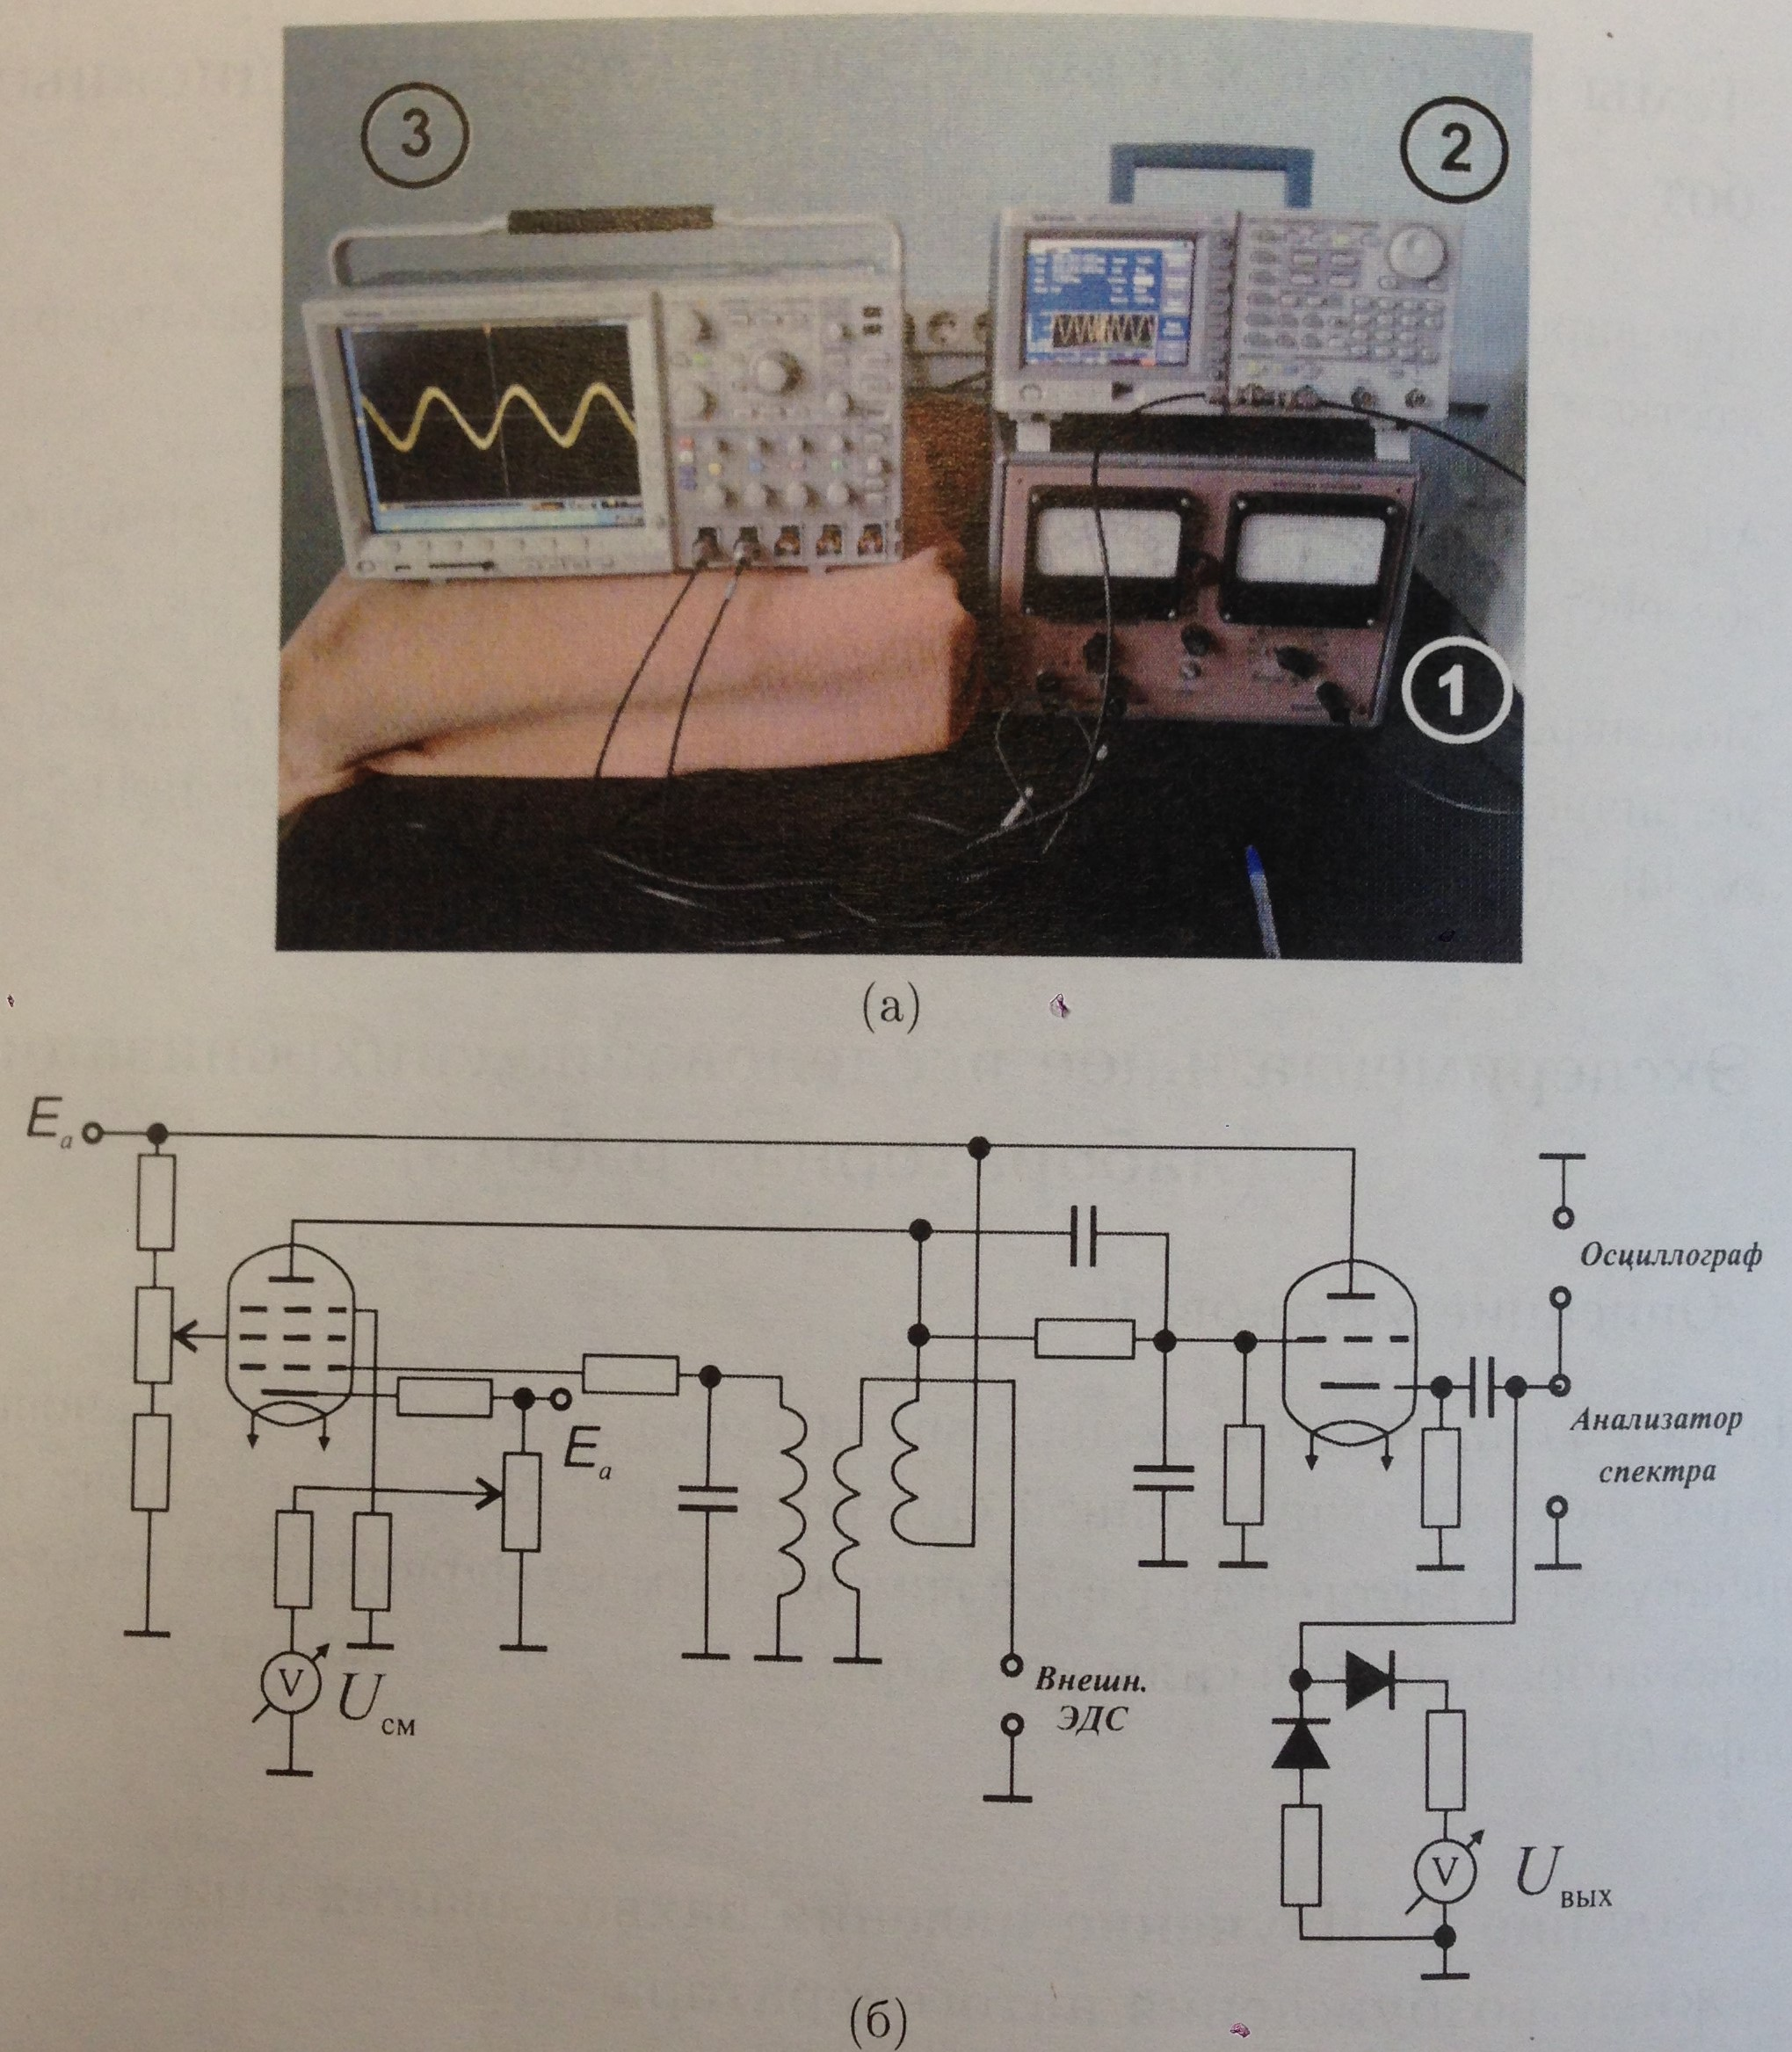
\includegraphics[width=0.8\linewidth]{photo/IMG_9783}
	\caption{схема установки}
	\label{pic.1}
\end{figure}
%\subsection*[Задание 1]{Изучение явления захватывания при мягком режиме возбуждения автогенератора}
\subsection*{Изучение явления захватывания при мягком режиме возбуждения автогенератора}
\begin{enumerate}
	\item 
	Установили мягкий режим автономного генератора путем подбора напряжения на управляющей сетки лампы $U\text{см}=0,6\:\text{В}$. Измерили амплитуду и частоту полученных автоколебаний $A=2\:\text{В}$, $f=426\:\text{кГц}$.
	\item
	Не меняя параметров схемы, подали внешнее воздействие. Сняли АЧХ для различных амплитуд внешнего сигнала. 
%	\begin{figure}[H]
%		\centering
%		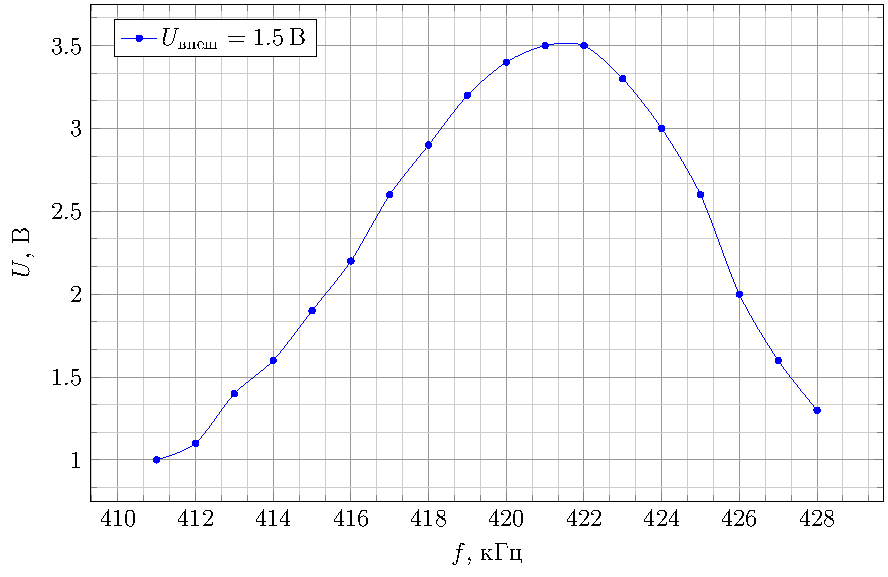
\includegraphics[width=0.7\linewidth]{plots/fig2_1}
%	\end{figure}
%	\begin{figure}[H]
%	\centering
%	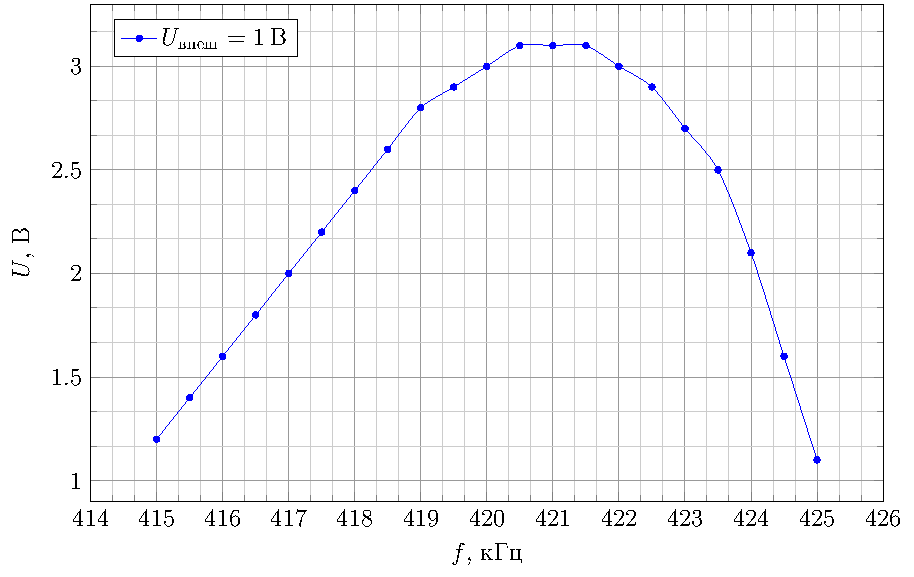
\includegraphics[width=0.7\linewidth]{plots/fig2_2}
%	\end{figure}
%\begin{figure}[H]
%	\centering
%	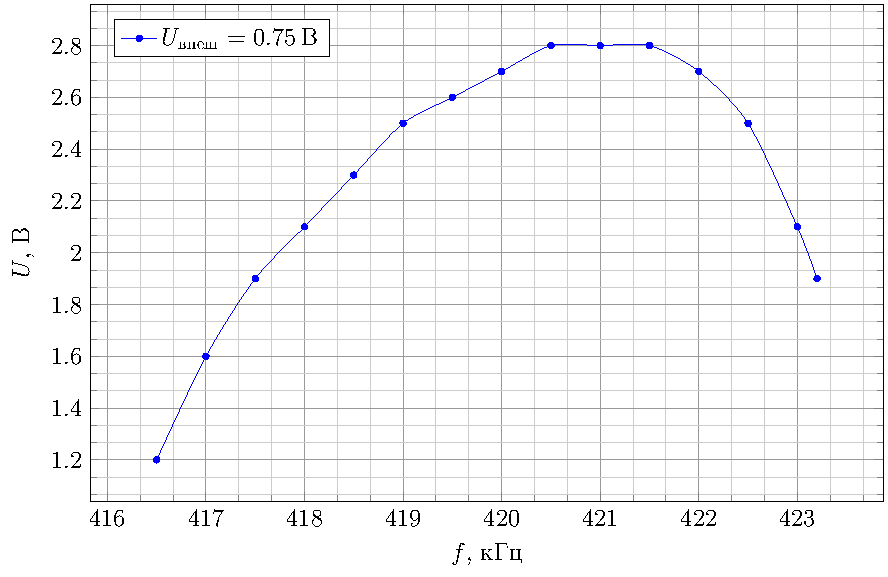
\includegraphics[width=0.7\linewidth]{plots/fig2_3}
%\end{figure}
%\begin{figure}[H]
%	\centering
%	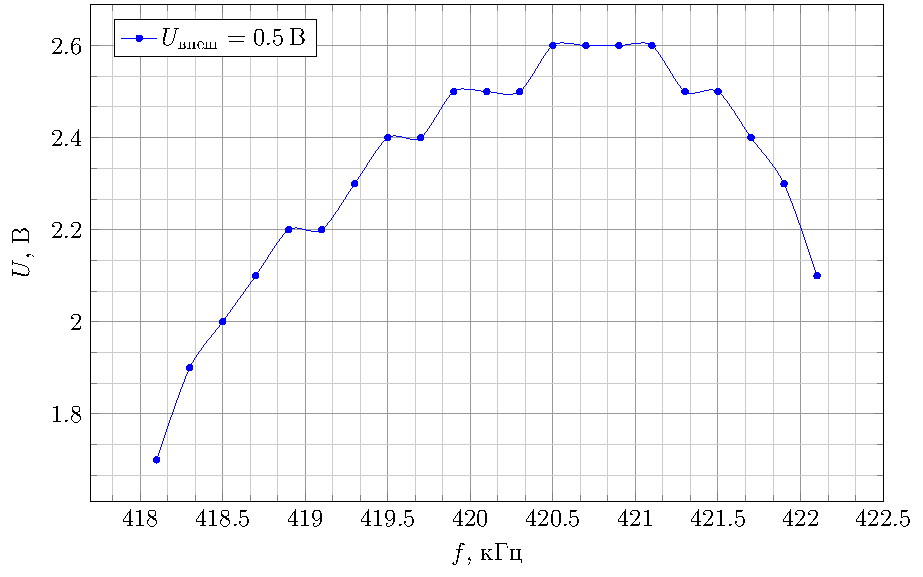
\includegraphics[width=0.7\linewidth]{plots/fig2_4}
%\end{figure}
\begin{figure}[H]
	\centering
	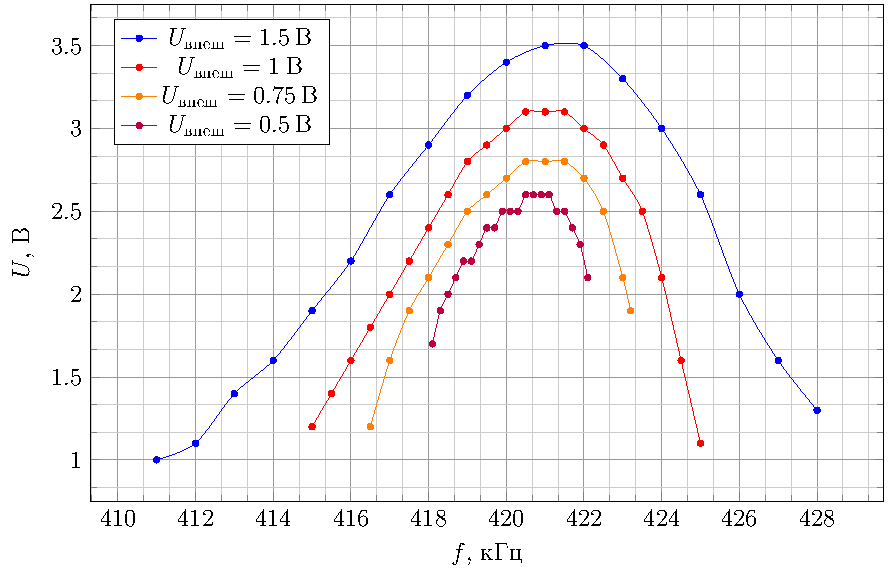
\includegraphics[width=\linewidth]{plots/fig2_comm}
\end{figure}
	\item
	Сняли зависимости значений левой и правой границ полосы синхронизации от амплитуды внешнего сигнала при фиксированных значениях параметров автономного генератора. Проанализировали зависимость ширины полосы синхронизации от амплитуды внешней силы.
	 \begin{figure}[H]
	 	\centering
	 	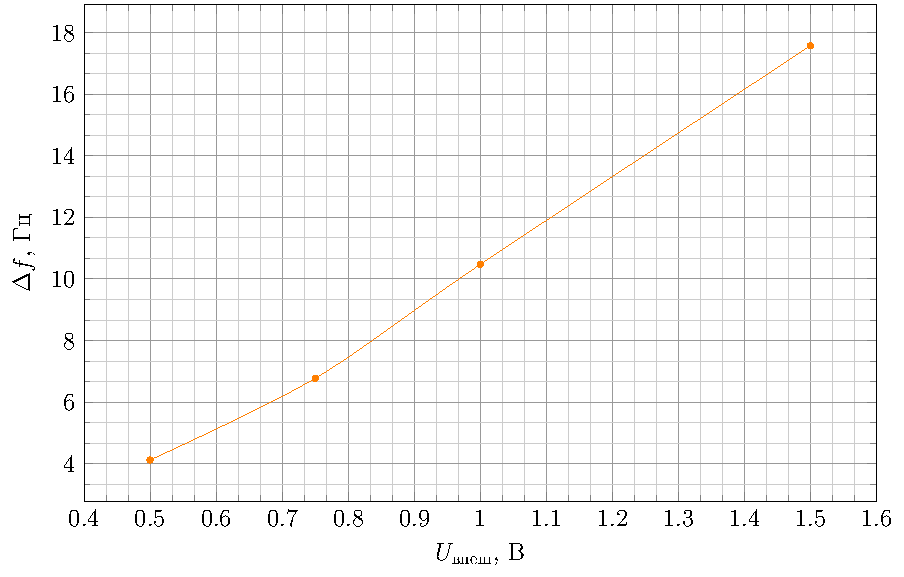
\includegraphics[width=0.8\linewidth]{plots/fig3}
	 \end{figure}
 	При увеличении амплитуды внешнего сигнала, ширина полосы синхронизации также возрастает.
 	\item 
 	Сняли зависимости значений левой и правой границ полосы захвата в режим синхронизации от амплитуды внешней силы при фиксированной амплитуде автономного генератора. Рассчитали ширину полосы захвата, проанализировали зависимость ширины полосы захвата в синхронный режим от амплитуды внешней силы.
 	\begin{figure}[H]
 		\centering
 		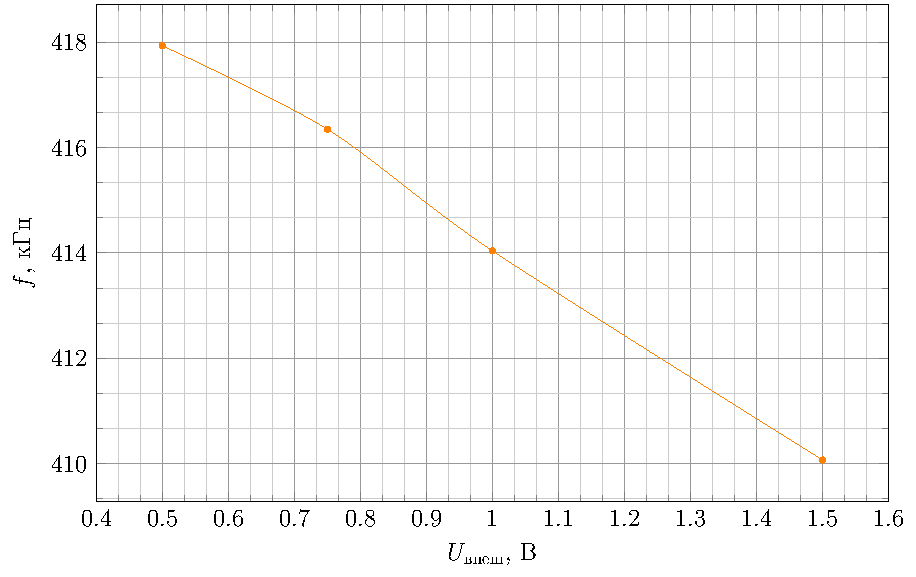
\includegraphics[width=0.8\linewidth]{plots/fig4_1}
 	\end{figure}
  	\begin{figure}[H]
 	\centering
 	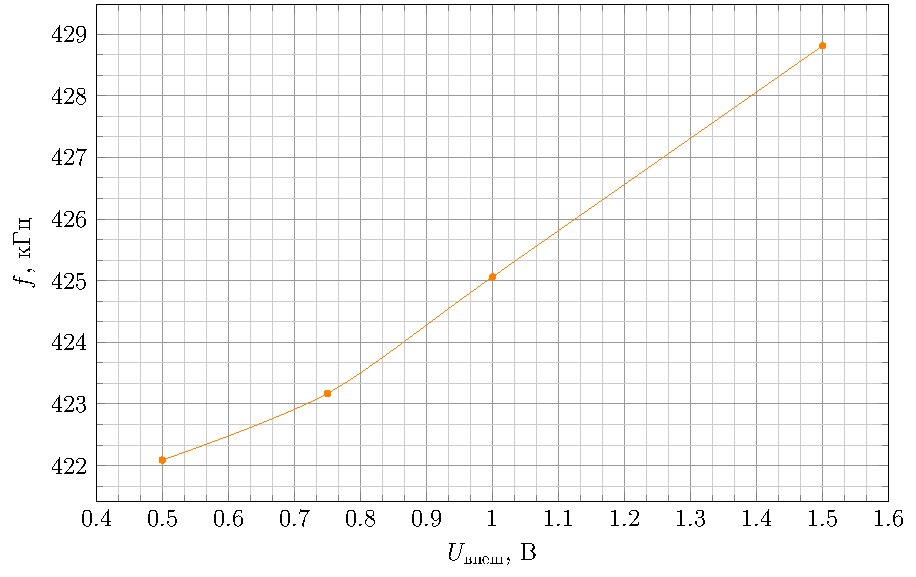
\includegraphics[width=0.8\linewidth]{plots/fig4_2}
 	\end{figure}
 При увеличении амплитуды внешнего сигнала левая и правая граница полосы захвата уменьшаются по величине.
 	\item 
 	Сравнили полосы синхронизации и захвата при нескольких фиксированных значениях амплитуды внешней силы. 
  	\begin{figure}[H]
	\centering
	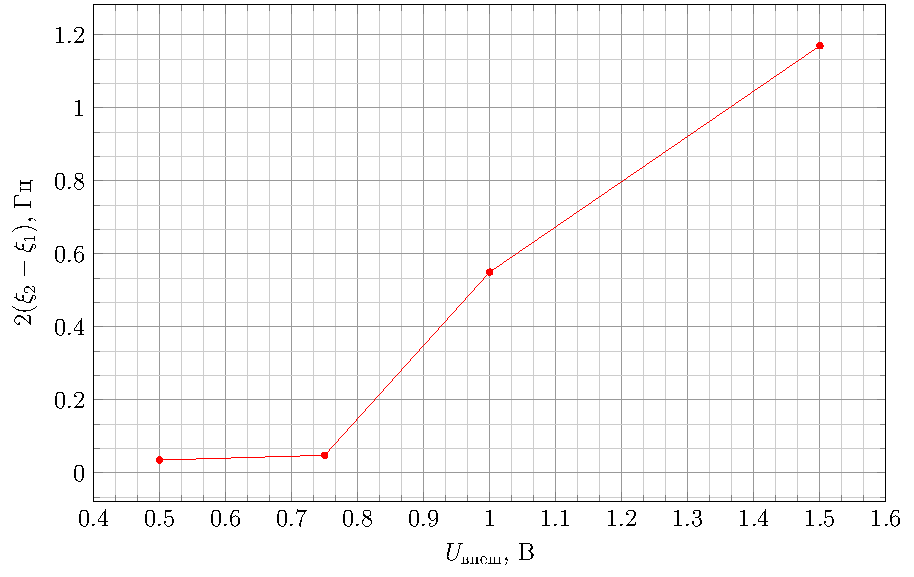
\includegraphics[width=0.8\linewidth]{plots/fig5}
 	\end{figure}
 где $\xi_2$ и $\xi_1$ правые границы полосы удержания и полосы синхронизации соответственно.
 При уменьшении амплитуды внешнего сигнала разность полосы удержания и полосы синхронизации уменьшается.
 	\item 
 	Сняли зависимости амплитуды колебаний в синхронном режиме на левой границе полосы синхронизации. 
 	\begin{figure}[H]
 		\centering
 		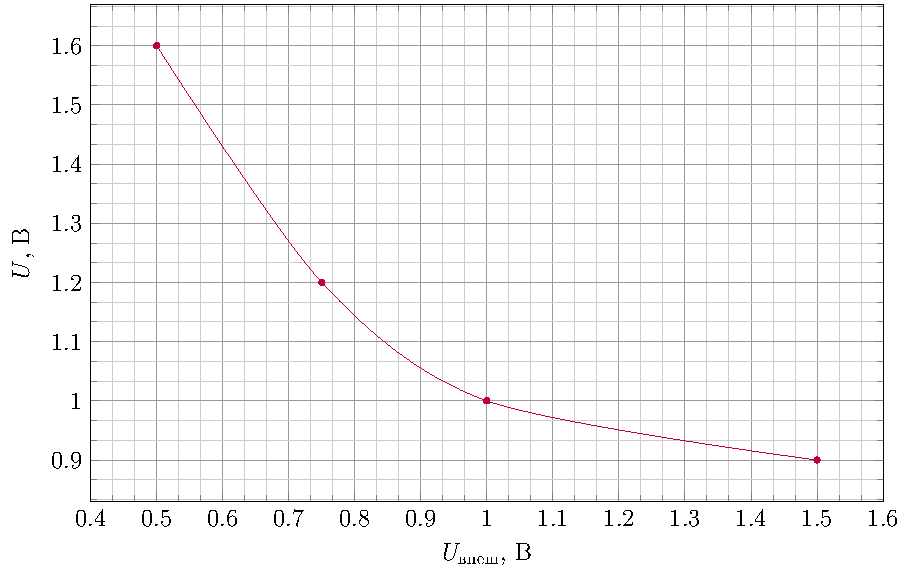
\includegraphics[width=0.8\linewidth]{plots/fig6}
 	\end{figure}
 Сфотографировали осциллограммы режима биений в окрестности границы полосы синхронизации для слабого и сильного сигналов.
 \begin{figure}[H]
 	\centering
 	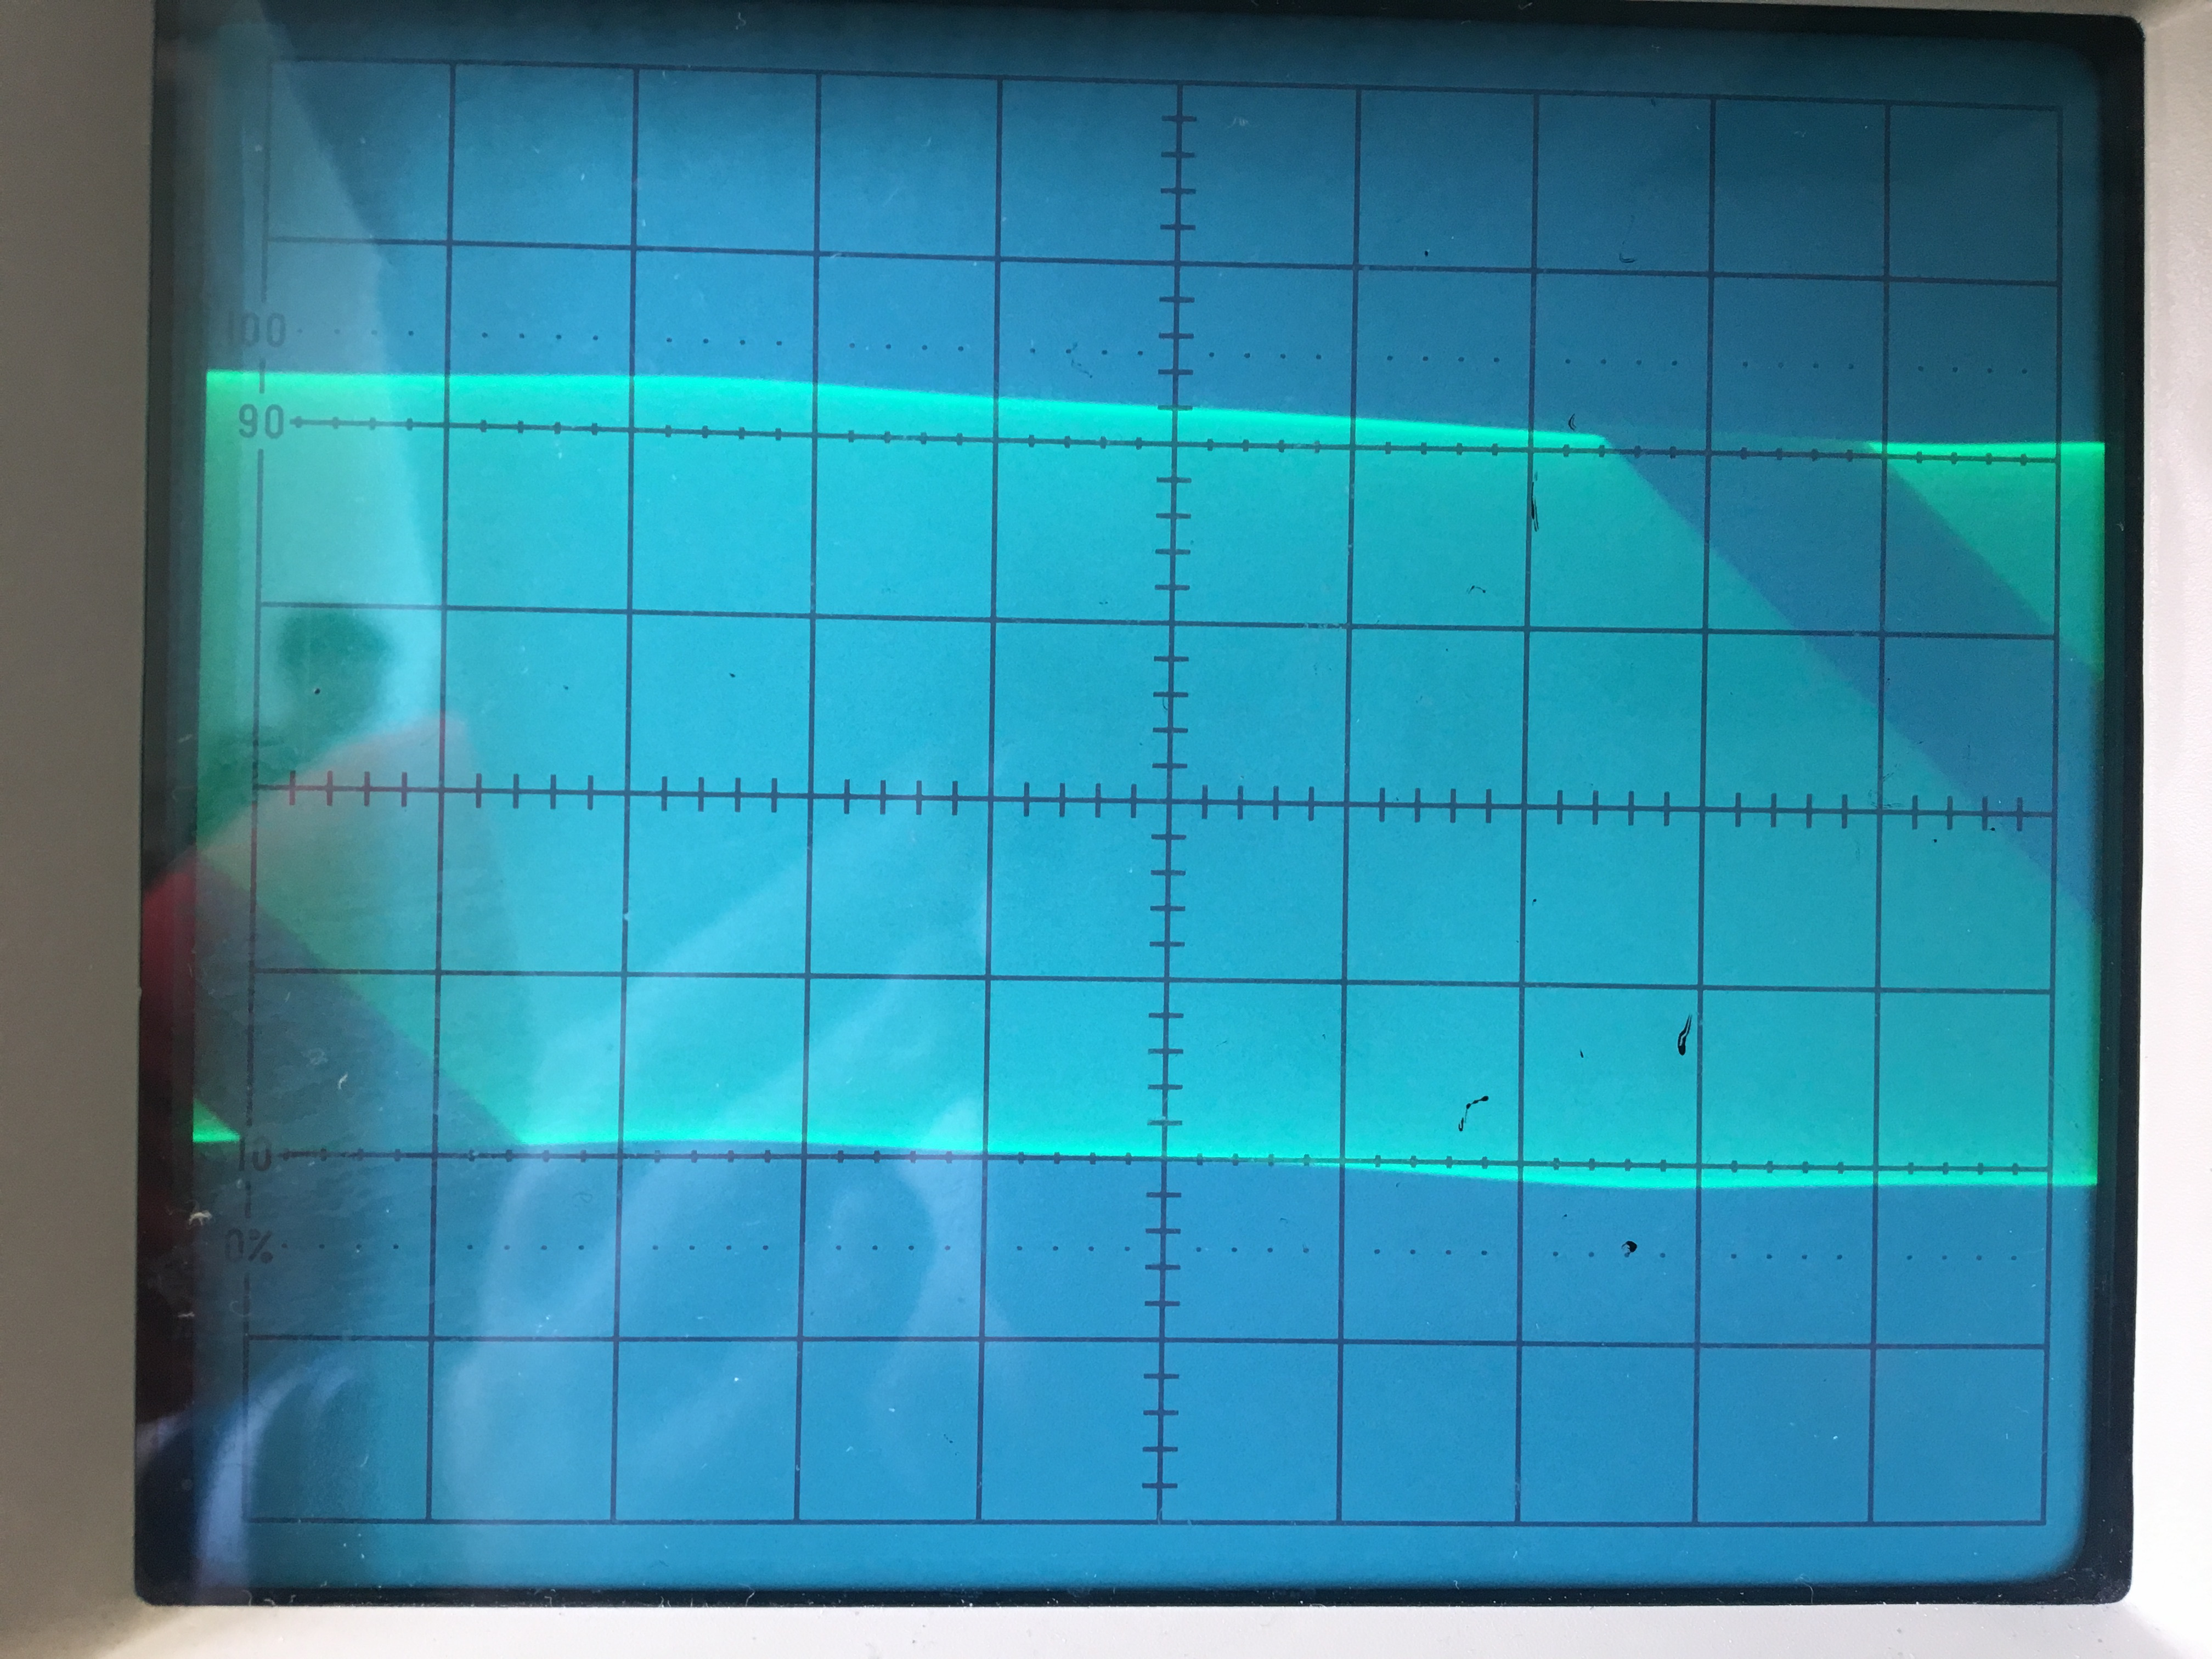
\includegraphics[width=0.8\linewidth]{photo/IMG_3224}
 \end{figure}
\begin{figure}[H]
	\centering
	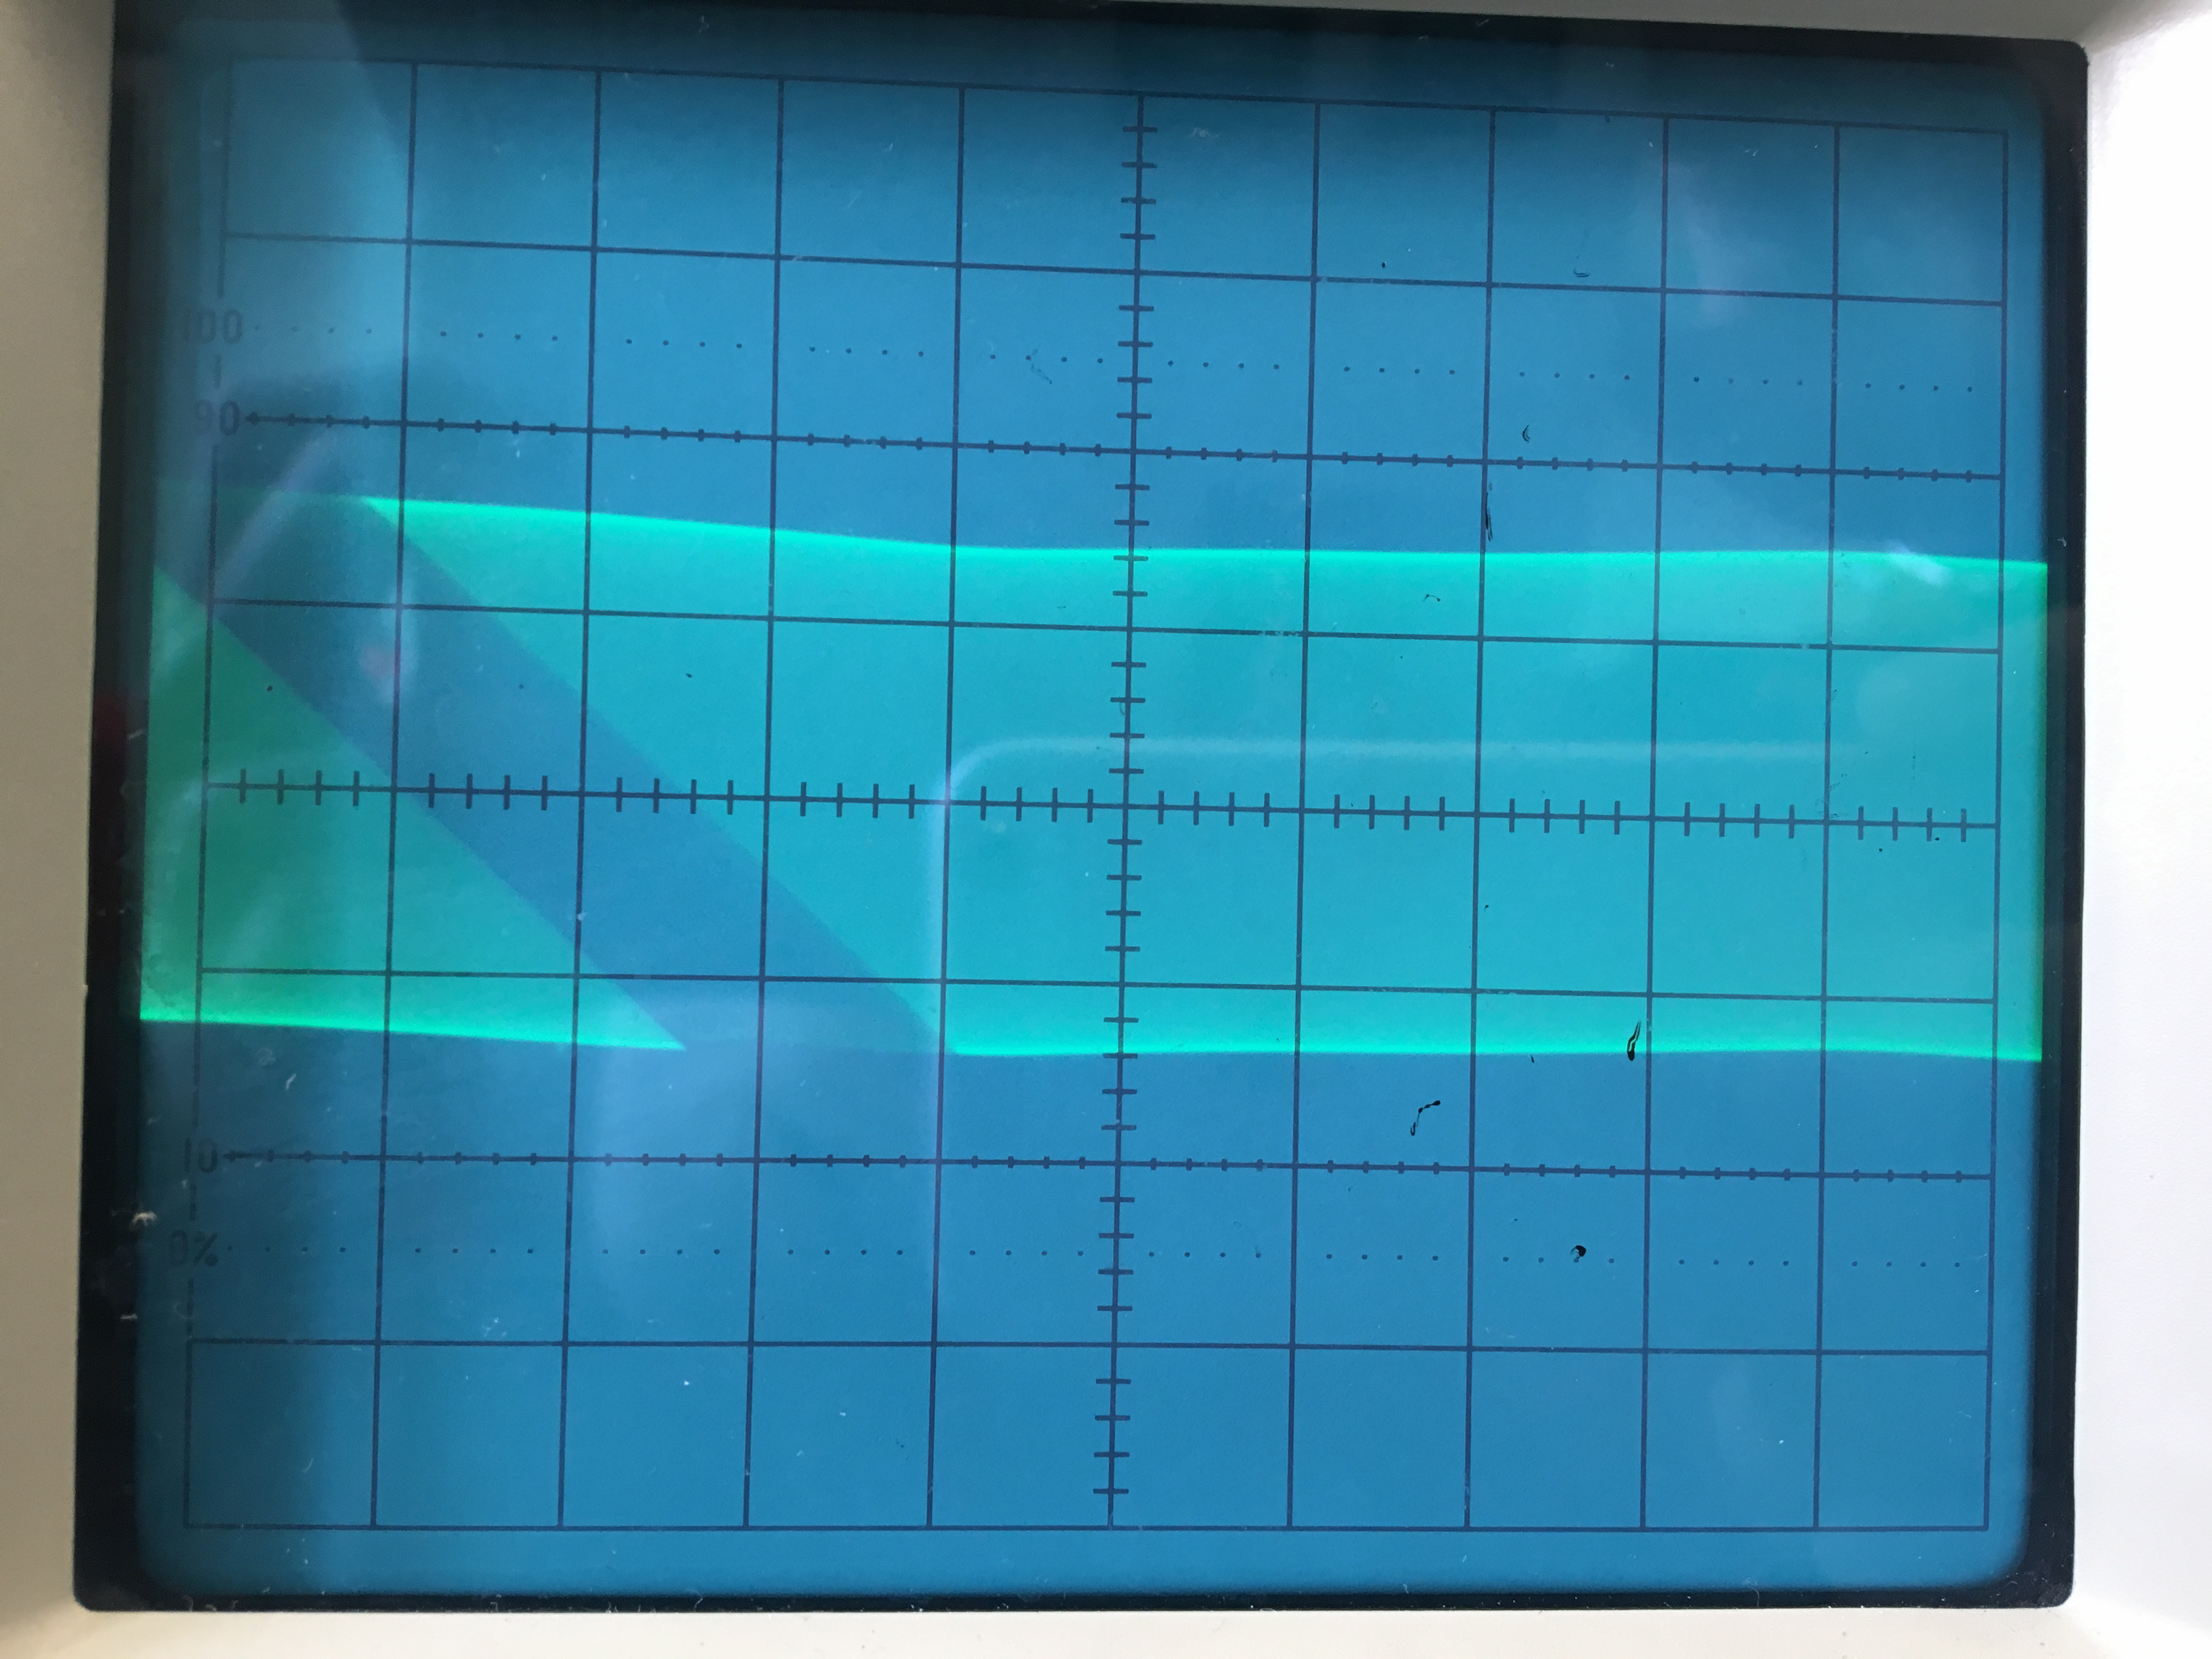
\includegraphics[width=0.8\linewidth]{photo/IMG_3226}
\end{figure}
\begin{figure}[H]
	\centering
	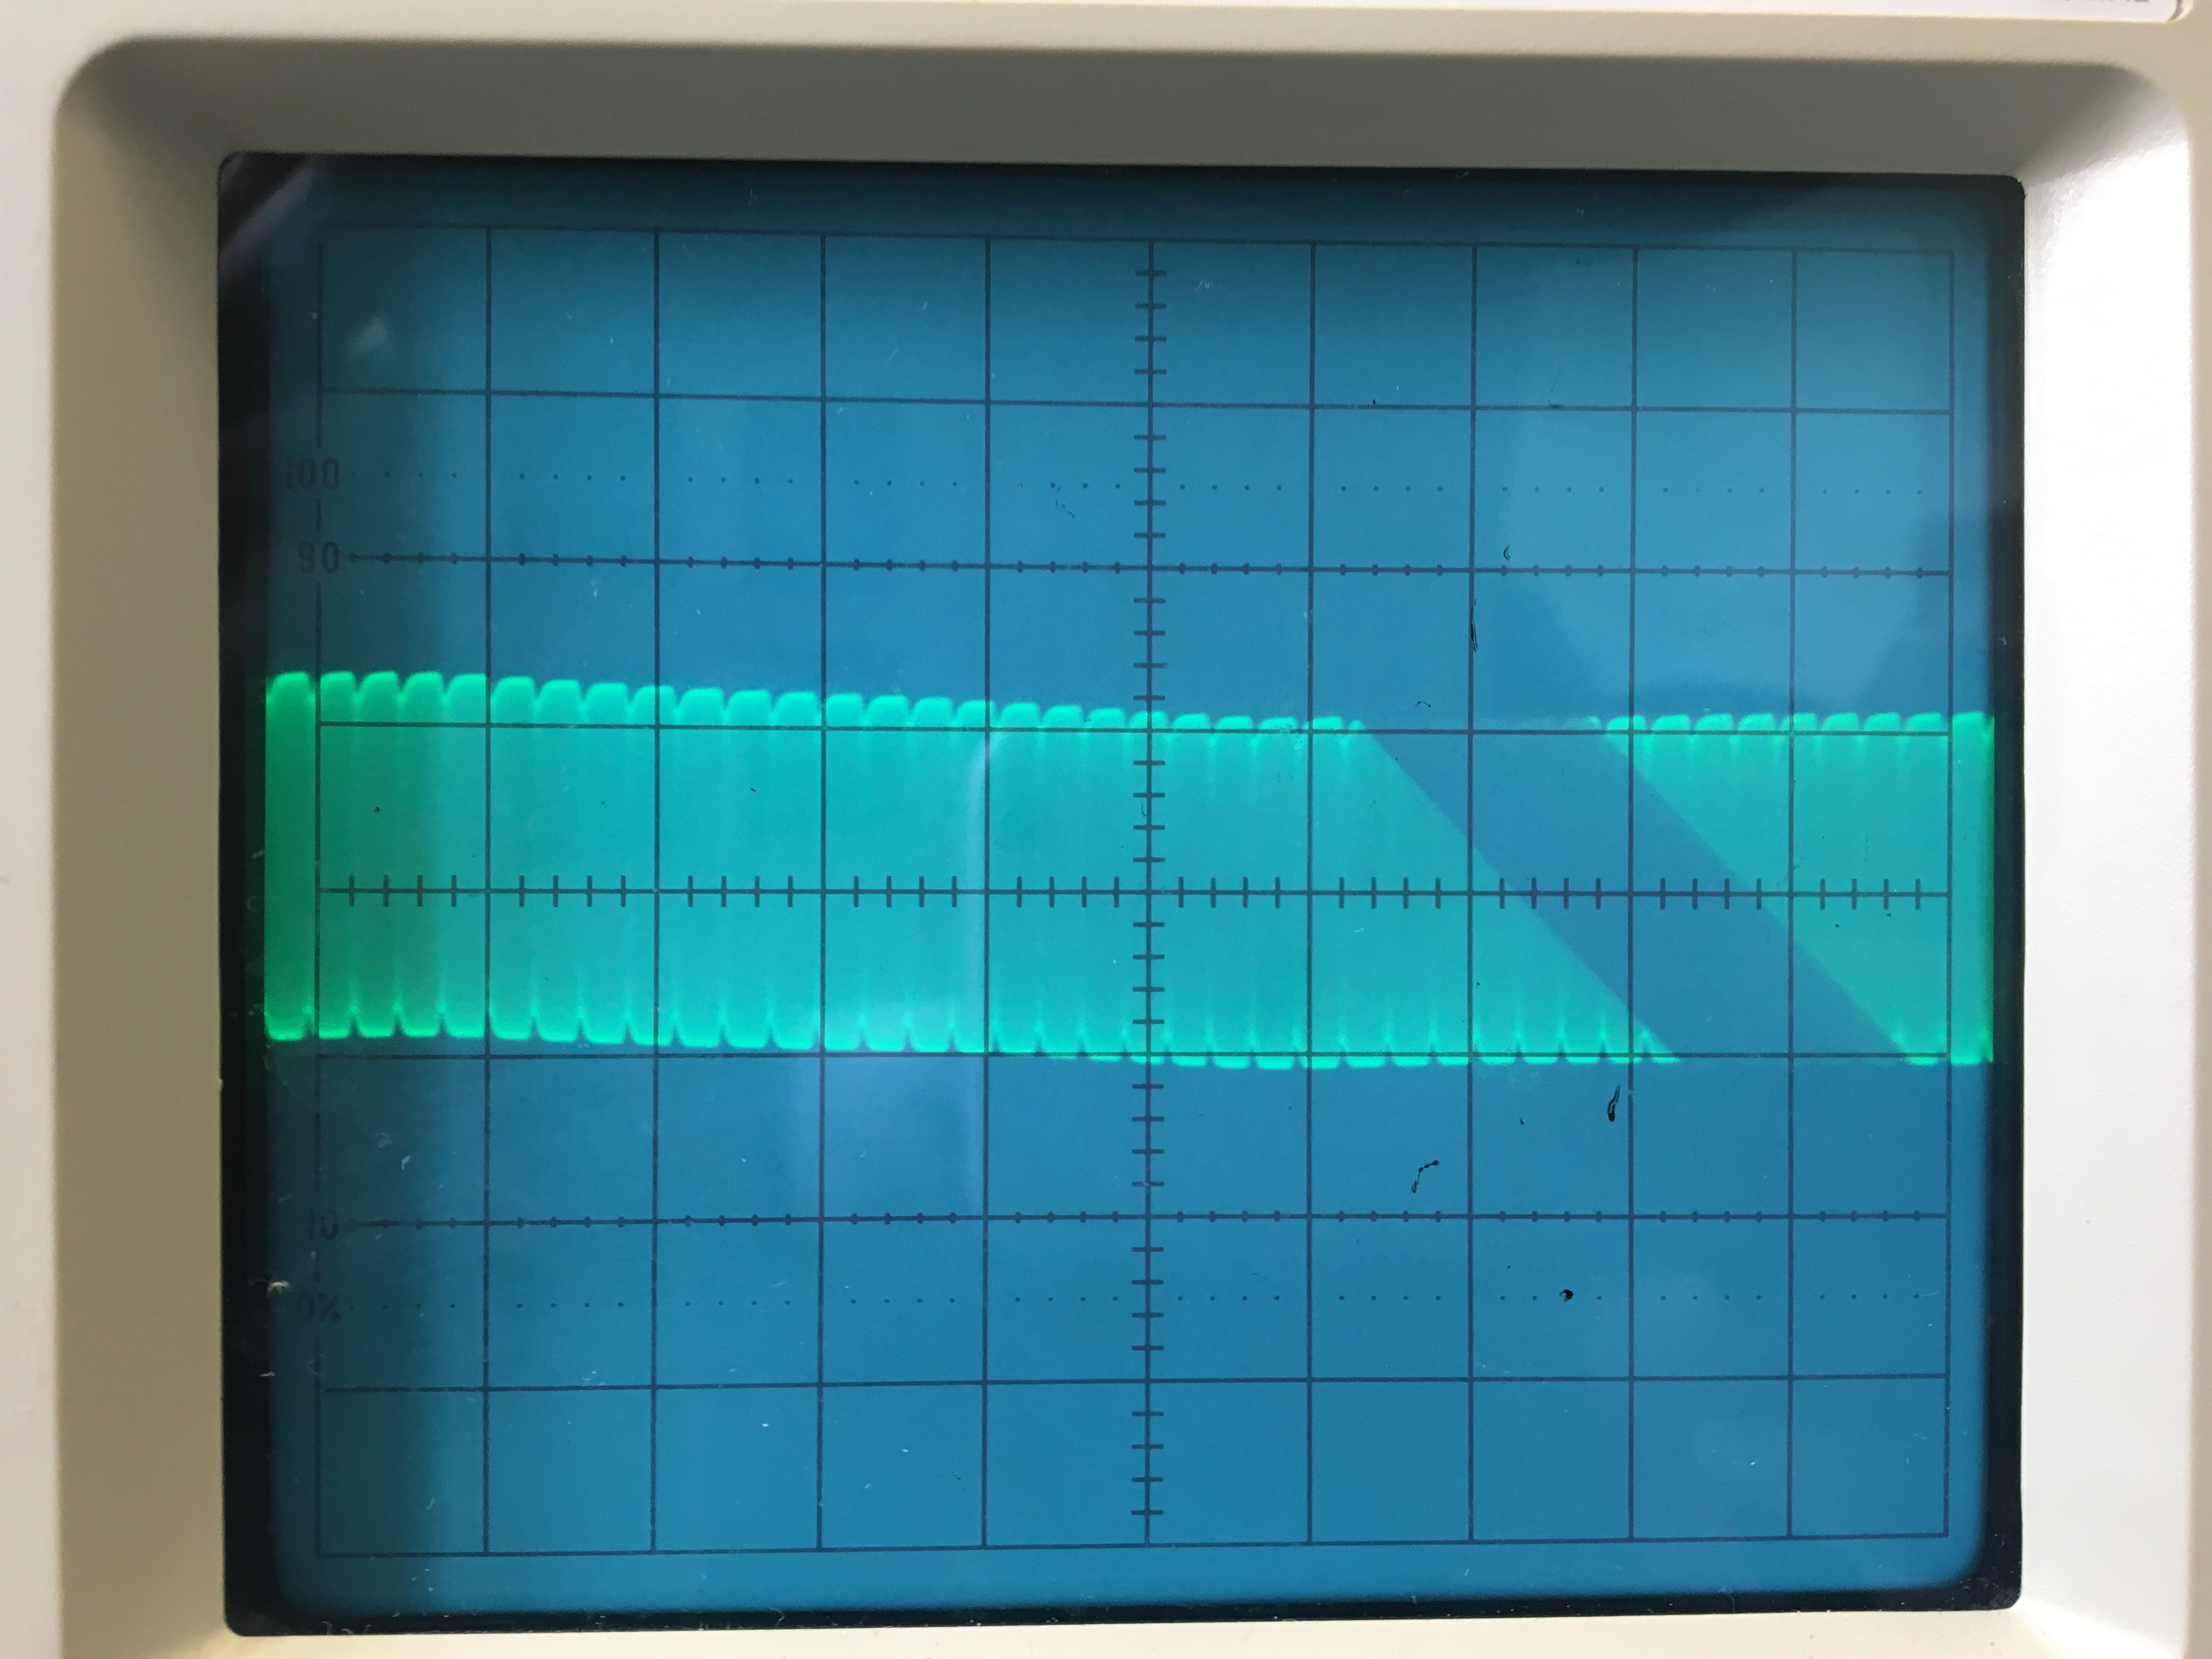
\includegraphics[width=0.8\linewidth]{photo/IMG_3228}
\end{figure}
\begin{figure}[H]
	\centering
	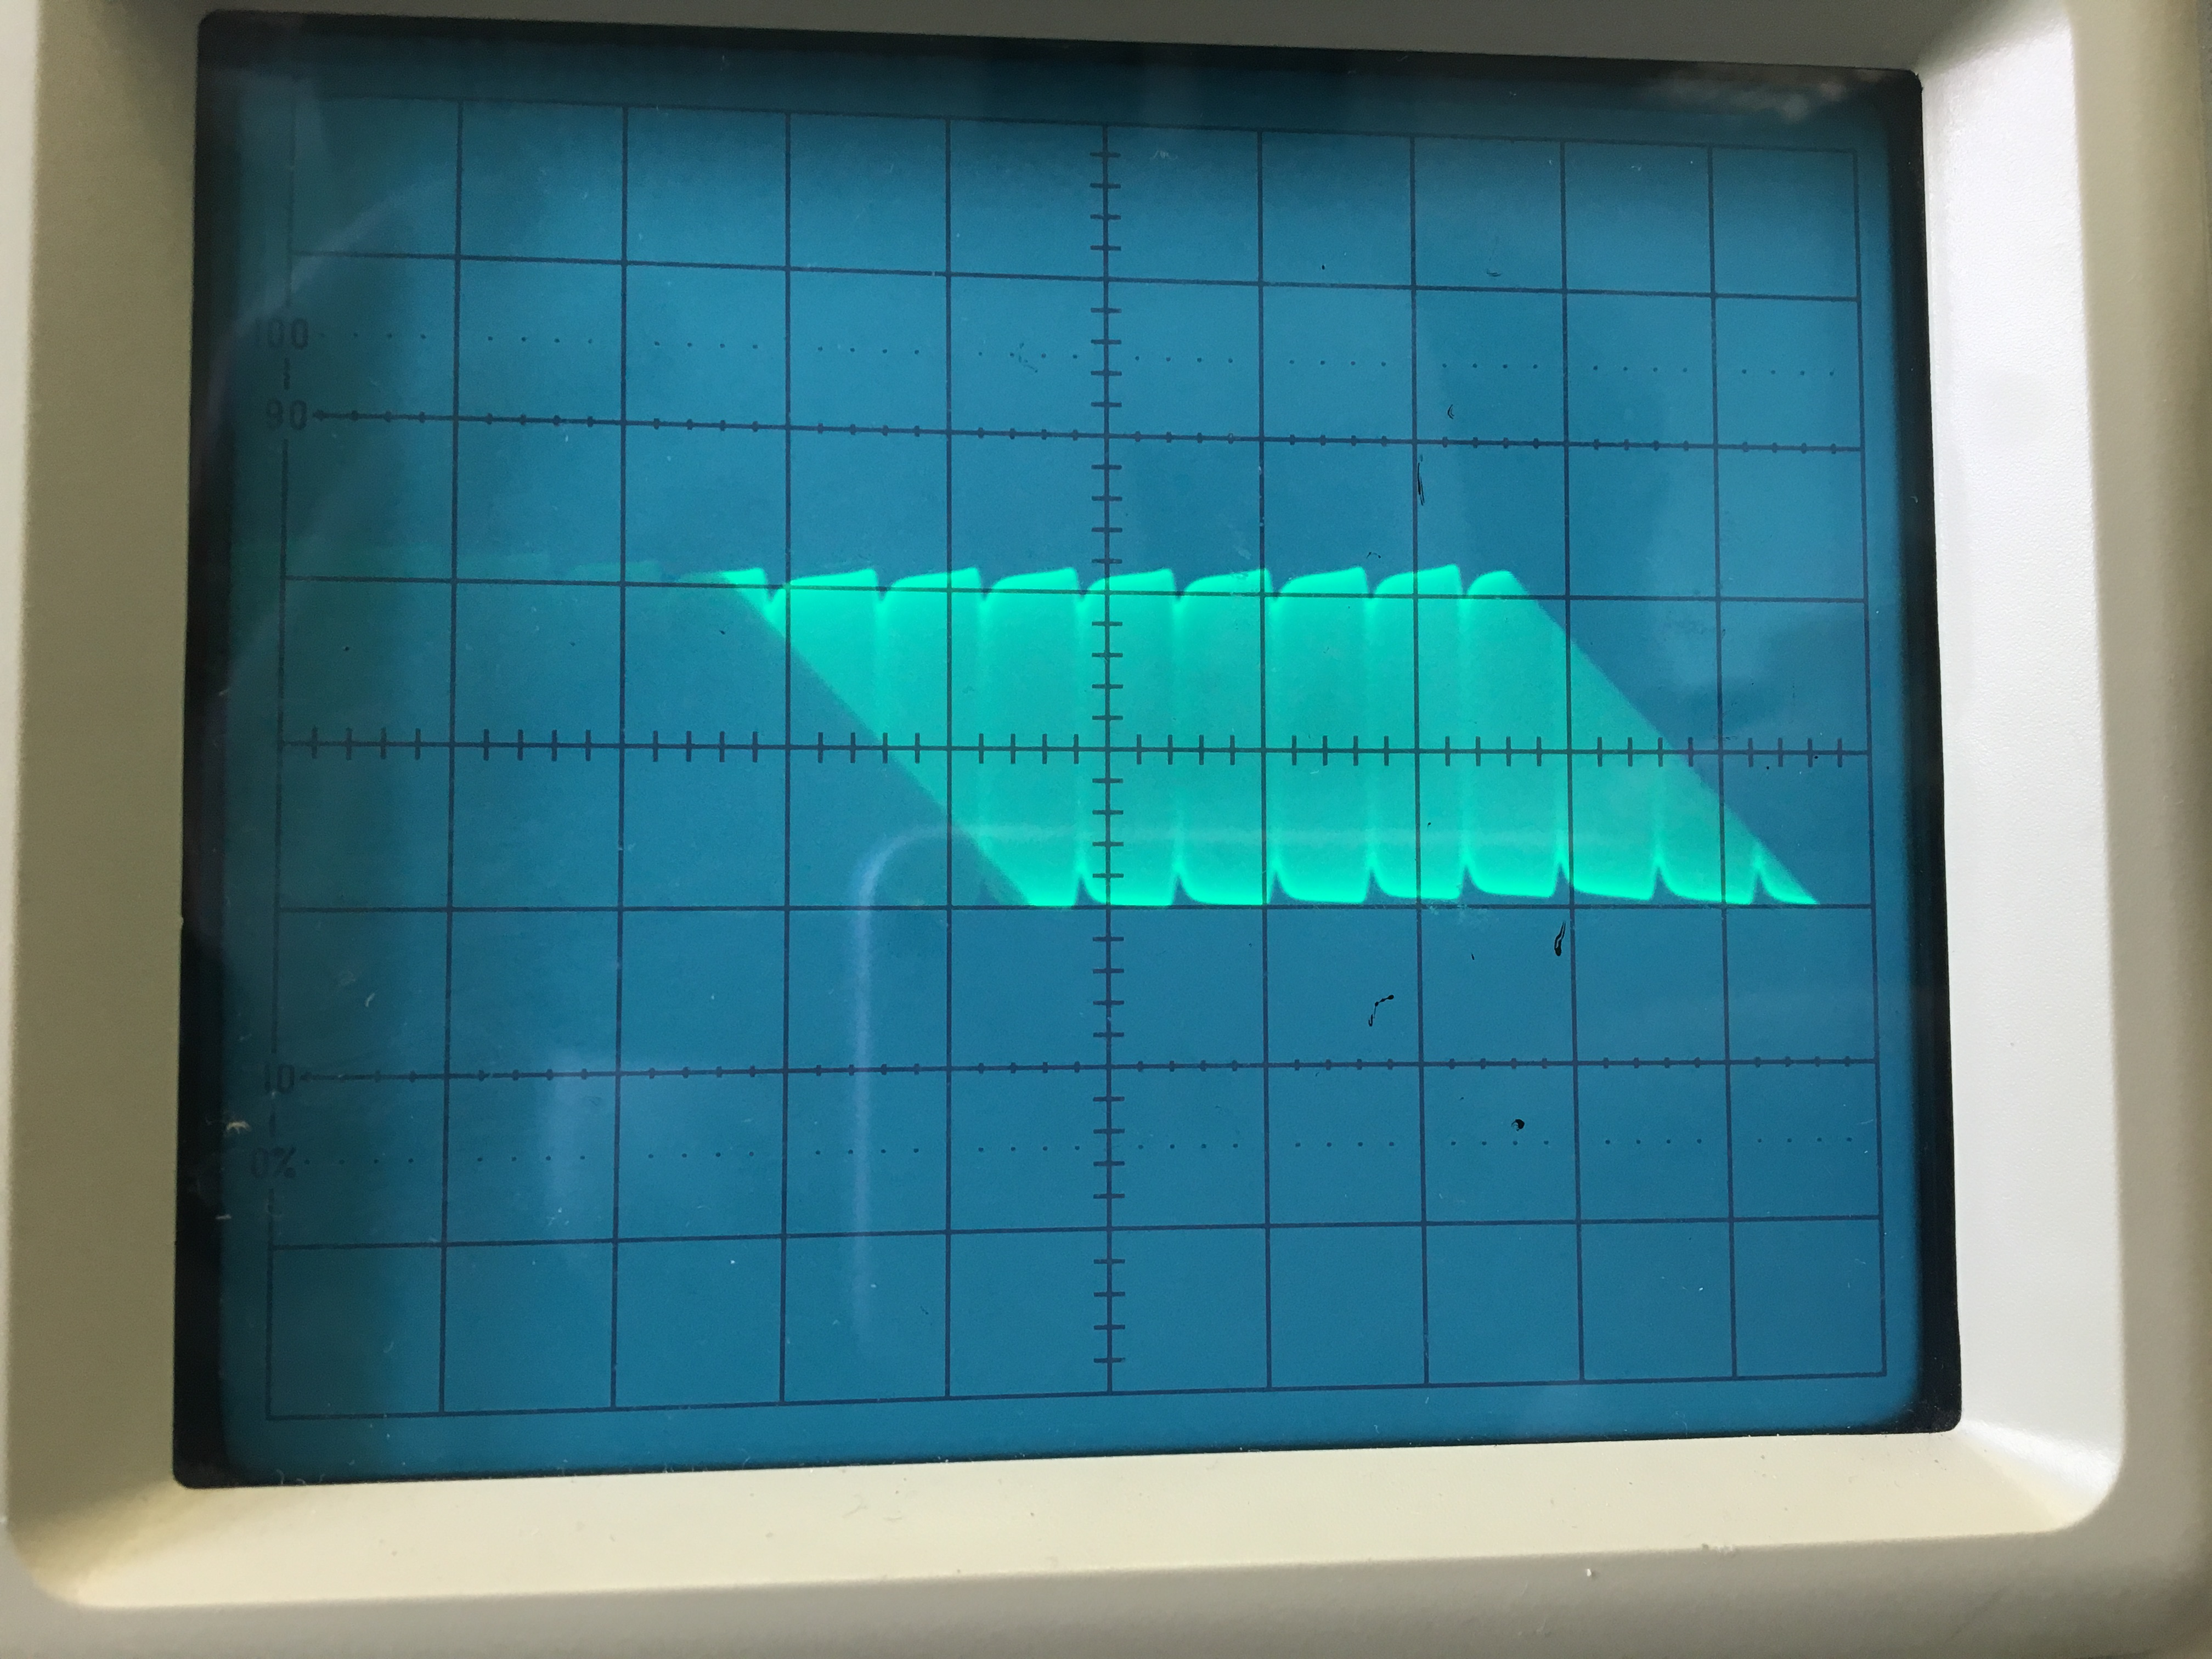
\includegraphics[width=0.8\linewidth]{photo/IMG_3230}
\end{figure}
Из полученных осциллограмм можно сделать вывод, что граница слабого сигнала лежит в пределах напряжений $0.75\text{В}<U_\text{внеш}<1\text{В}$ внешнего сигнала.
\end{enumerate}
\subsection*{Изучение явления захватывания при жестком режиме возбуждения}
\begin{enumerate}
	\item 
	Подобрали параметры автономного генератора так, чтобы осуществлялся жесткий режим возбуждения.
	Напряжение смещения $U_\text{см}=3\:\text{В}$, величина обратной связи 45. Бифуркационные параметры обратной связи принимают значения 30 и 80.
	\item
	Для жесткого режима возбуждения сняли семейство АЧХ для различных амплитуд внешнего сигнала. 
	\begin{figure}[H]
		\centering
		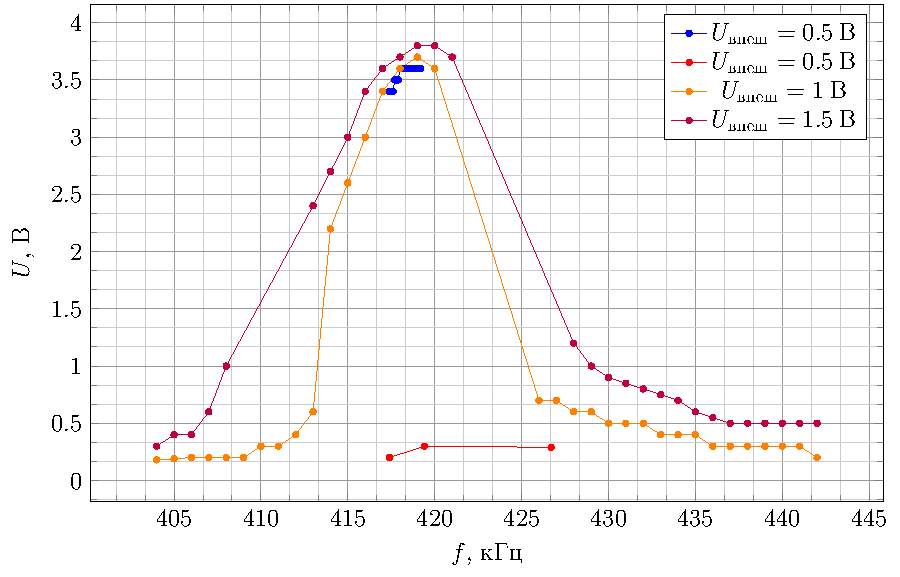
\includegraphics[width=\linewidth]{plots/fig3_2a}
	\end{figure}
	Сравнили полученные АЧХ с АЧХ для мягкого режима.
	\begin{figure}[H]
		\centering
		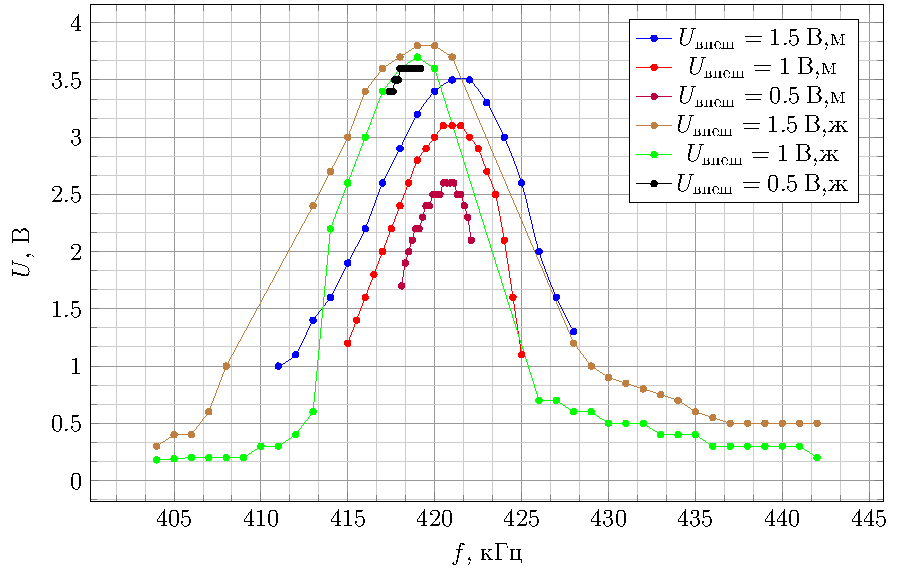
\includegraphics[width=\linewidth]{plots/fig3comm}
	\end{figure}
\end{enumerate} 
\end{document}